\section{Matrices}

A vector can be multiplied by a matrix as follows.
%
\[
\begin{bmatrix}
    a & b\\
    c & d
\end{bmatrix}
\begin{bmatrix}
    x \\ y
\end{bmatrix}
=
\begin{bmatrix}
    ax + by\\
    cx + dy
\end{bmatrix}
\]

Figure \ref{fig:Ch04-matrix-vector-mult} shows a diagrammatic representation of this procedure.

\begin{figure}[H]
    \centering

    \begin{tikzpicture}[scale=1]
        \node at (0,0) {\(
            \begin{bmatrix}
                a & b\\
                c & d
            \end{bmatrix}
            \overset{{\color{gray}
                \begin{bmatrix}
                    x \\ y
                \end{bmatrix}
            }}{
                \begin{bmatrix}
                    x \\ y
                \end{bmatrix}
            }
            =
            \begin{bmatrix}
                ax + by\\
                cx + dy
            \end{bmatrix}
        \)};

        \draw[line width=1pt, -stealth, BrickRed] (-0.8, 0.7) arc (90:180:0.75 and 0.7);
        \draw[line width=1pt, -stealth, BrickRed] (-0.8, 0.3) arc (90:180:0.25 and 0.3);
    \end{tikzpicture}
    
    \caption{Multiplying a matrix by a vector.}
    \label{fig:Ch04-matrix-vector-mult}
\end{figure}

Notice how a matrix maps a vector, \(\begin{bmatrix} x \\ y \end{bmatrix}\), to a new one, \(\begin{bmatrix} ax + by\\ cx + dy \end{bmatrix}\), just like a linear map does. This is not a coincidence --- it is in fact possible to express any linear map as a matrix, as we shall see below.





\subsection{Expressing linear maps as matrices}

Consider two vector spaces:
%
\begin{itemize}
    \item A vector space \(U\) of \(n\) dimensions, with a specified set of basis vectors.
    \item A vector space \(V\) of \(m\) dimensions, with a specified set of basis vectors.
\end{itemize}
%
Every linear map \(f : U \to V\) can then be represented by a matrix \(M\) with \(m\) rows and \(n\) columns. Each column represents the image of a basis vector of \(U\), expressed in the basis of \(V\).

It's important to take a moment to digest what this means. Several examples are included below.



\subsubsection{Example 1: An endomorphism with unchanged bases}

\vspace{15pt}
\begin{mdframed}[linewidth=1pt]
\noindent \textbf{Setup.} We set both \(U\) and \(V\) to \(\mathbb{R}^2\). We will use the canonical basis for both vector spaces:
%
\[
\left\{
    \begin{bmatrix}
        1 \\ 0
    \end{bmatrix},
    \begin{bmatrix}
        0 \\ 1
    \end{bmatrix}
\right\}\text{.}
\]

We define \(f\) to be a linear map that scales the length of a vector by a factor of \(1.5\) and then rotates it by \(30\degree\). See figure \ref{fig:Ch04-example-1}.

We want to find the matrix \(M\) that represents this endomorphism.

\begin{figure}[H]
    \centering

    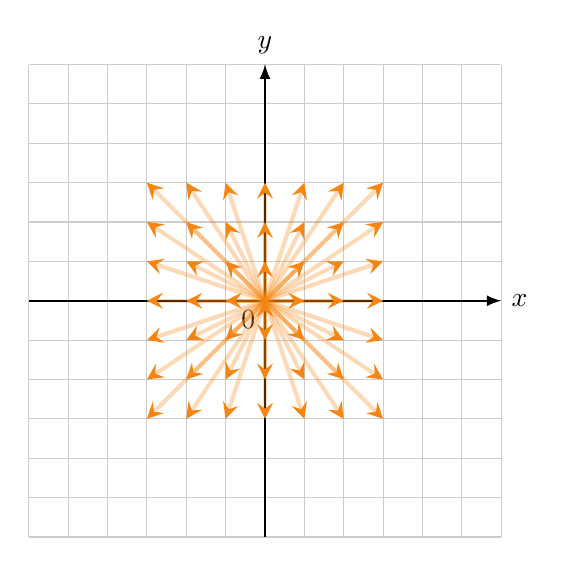
\begin{tikzpicture}[scale=0.5]
        \draw[thin,gray!40] (-6,-6) grid (6, 6);
        \draw[thick, ->, >=latex] (-6,0)--(6,0) node[right]{\(x\)};
        \draw[thick, ->, >=latex] (0,-6)--(0,6) node[above]{\(y\)};
        \draw (0, 0) node[below left] {0};
        
        \foreach \x in {-3,...,3} {
            \foreach \y in {-3,...,3} {
                \draw[line width=1.5pt, BurntOrange, -stealth, draw opacity=0.3] (0,0)--(\x,\y);
            }
        }
    \end{tikzpicture}

    \begin{tikzpicture}[scale=0.5]
        \draw[thin,gray!40] (-6,-6) grid (6, 6);
        \draw[thick, ->, >=latex] (-6,0)--(6,0) node[right]{\(x\)};
        \draw[thick, ->, >=latex] (0,-6)--(0,6) node[above]{\(y\)};
        \draw (0, 0) node[below left] {0};
        
        \foreach \x in {-3,...,3} {
            \foreach \y in {-3,...,3} {
                \draw[line width=1.5pt, Fuchsia, -stealth, draw opacity=0.3] (0,0) -- ($1.5*({cos(30) * \x + cos(120) * \y}, {sin(30) * \x + sin(120) * \y})$);
            }
        }
    \end{tikzpicture}
    
    \caption{The linear map \(f\) takes a vector (in orange) and scales it by a factor of \(1.5\) before rotating it by \(30\degree\) anticlockwise. This results in a new vector (in purple).}
    \label{fig:Ch04-example-1}
\end{figure}

\vspace{2pt}
\end{mdframed}


Let's start with the size of the matrix, also known as its \textit{order}. We know both \(U\) and \(V\) are 2-dimensional vector spaces, so the matrix is going to have an order of \(2 \times 2\), with two rows and two columns.
%
\[
M = \begin{bmatrix}
    \color{BrickRed}\square & \color{MidnightBlue}\square\\
    \color{BrickRed}\square & \color{MidnightBlue}\square\\
\end{bmatrix}
\]

Remember that each column of the matrix represents the image of a basis vector of \(U\), expressed in the basis of \(V\). This means that the first column (in red) will represent where the first basis vector of \(U\) will get mapped to, as expressed using the basis vectors of \(V\).
%
\begin{itemize}
    \item The first basis vector of \(U\) is \(\begin{bmatrix} 1 \\ 0 \end{bmatrix}\). Following the rule of our transformation, the linear map will take us to \(\begin{bmatrix} 2\cos{30\degree} \\ 2\sin{30\degree} \end{bmatrix}\). Since the bases are the same for both vector spaces, this will be the first column of our matrix \(M\).
    \item Similarly, the second basis vector of \(U\) is \(\begin{bmatrix} 0 \\ 1 \end{bmatrix}\). This maps to \(\begin{bmatrix} 2\cos{120\degree} \\ 2\sin{120\degree} \end{bmatrix}\), or \(\begin{bmatrix} -2\sin{30\degree} \\ 2\cos{30\degree} \end{bmatrix}\). Again, the bases are the same for both vector spaces, so this will be the second column of our matrix \(M\).
\end{itemize}
%
Hence, the linear map \(f\) is represented by the matrix
%
\[
M = \begin{bmatrix}
    2\cos{30\degree} & -2\sin{30\degree}\\
    2\sin{30\degree} & 2\cos{30\degree}
\end{bmatrix}
%
= \begin{bmatrix}
    \sqrt{3} & -1\\
    1 & \sqrt{3}
\end{bmatrix}
\]
%
and this matrix can be applied to any vector in \(U\). For instance, consider the input vector \(\vec{v} = \begin{bmatrix} 3 \\ 2 \end{bmatrix}\). To find out what this vector maps to, we simply work out the following expression:
%
\begin{align*}
    M\vec{v} &= \begin{bmatrix}
        \sqrt{3} & -1\\
        1 & \sqrt{3}
    \end{bmatrix}
    \begin{bmatrix} 3 \\ 2 \end{bmatrix}\\
    %
    &= \begin{bmatrix}
        3\sqrt{3} - 2\\
        2\sqrt{3} + 3
    \end{bmatrix}
\end{align*}
%
to get our answer. This is verified in figure \ref{fig:Ch04-example-1-verification}.

\begin{figure}[H]
    \centering

    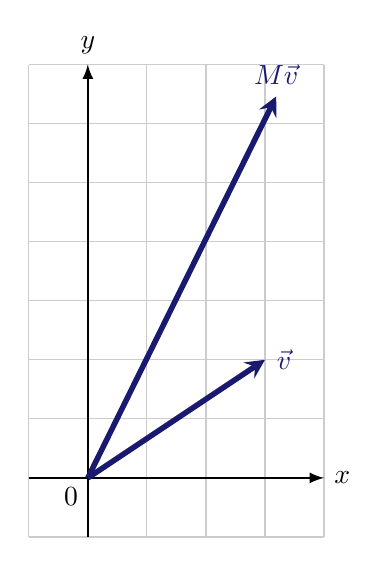
\begin{tikzpicture}[scale=0.75]
        \draw[thin,gray!40] (-1,-1) grid (4, 7);
        \draw[thick, ->, >=latex] (-1,0)--(4,0) node[right]{\(x\)};
        \draw[thick, ->, >=latex] (0,-1)--(0,7) node[above]{\(y\)};
        \draw (0, 0) node[below left] {0};
        
        \draw[line width=2pt, MidnightBlue, -stealth] (0,0)--(3,2) node[right]{\(\vec{v}\)};
        \draw[line width=2pt, MidnightBlue, -stealth] (0,0)--(1.73*3-2, 1.73*2+3) node[above]{\(M\vec{v}\)};
    \end{tikzpicture}
    
    \caption{Verifying the equivalence between the linear map \(f\) and the matrix \(M = \begin{bmatrix} \sqrt{3} & -1 \\ 1 & \sqrt{3} \end{bmatrix}\) by using an example vector \(\vec{v} = \begin{bmatrix} 3 \\ 2 \end{bmatrix}\).}
    \label{fig:Ch04-example-1-verification}
\end{figure}




\subsubsection{Example 2: An endomorphism with changed bases}

\vspace{15pt}
\begin{mdframed}[linewidth=1pt]
\noindent \textbf{Setup.} Like the previous example, we set both \(U\) and \(V\) to \(\mathbb{R}^2\), and we want to find a matrix \(M\) that corresponds to a linear map \(f\) where vectors are scaled 1.5 times and rotated by \(30\degree\) anticlockwise.

Only this time, we will use the canonical basis for the vector space \(U\):
%
\[
\left\{
    \begin{bmatrix}
        1 \\ 0
    \end{bmatrix},
    \begin{bmatrix}
        0 \\ 1
    \end{bmatrix}
\right\}
\]
%
and the following basis for \(V\). (Note that this is a basis since the two vectors are linearly independent.)
%
\[
\left\{
    \begin{bmatrix}
        2 \\ 0
    \end{bmatrix},
    \begin{bmatrix}
        -1 \\ 1
    \end{bmatrix}
\right\}
\]

\vspace{2pt}
\end{mdframed}


The process is really the same. We know from the previous example that the canonical basis vectors will be mapped to \(\begin{bmatrix} \sqrt{3} \\ 1 \end{bmatrix}\) and \(\begin{bmatrix} -1 \\ \sqrt{3} \end{bmatrix}\) respectively. All we have to do now is to express these vectors using the basis of \(V\).

Let's take the first vector \(\begin{bmatrix} \sqrt{3} \\ 1 \end{bmatrix}\) as an example. We want to find scalars \(x_1\) and \(y_1\) such that
%
\[x_1 \begin{bmatrix} 2 \\ 0 \end{bmatrix} + y_1 \begin{bmatrix} -1 \\ 1 \end{bmatrix} = \begin{bmatrix} \sqrt{3} \\ 1 \end{bmatrix}\text{.}\]
%
This has the solution of \(x_1 = (\sqrt{3}+1)/2\) and \(y_1 = 1\). In other words, the image of our first basis vector can be expressed using the basis of \(V\) as \(\begin{bmatrix} (\sqrt{3}+1)/2 \\ 1 \end{bmatrix}\). This will be the first column of our matrix \(M\).

Similarly, we want to find scalars \(x_2\) and \(y_2\) such that
%
\[x_2 \begin{bmatrix} 2 \\ 0 \end{bmatrix} + y_2 \begin{bmatrix} -1 \\ 1 \end{bmatrix} = \begin{bmatrix} -1 \\ \sqrt{3} \end{bmatrix}\text{.}\]
%
This has the solution of \(x_2 = (\sqrt{3}-1)/2\) and \(y_2 = \sqrt{3}\). This gives us the second column of our matrix: \(\begin{bmatrix} (\sqrt{3}-1)/2 \\ \sqrt{3} \end{bmatrix}\).

Hence, the matrix that is equivalent to \(f\) is given by
%
\[
M = 
\begin{bmatrix}
    (\sqrt{3}+1)/2 & (\sqrt{3}-1)/2\\
    1 & \sqrt{3}
\end{bmatrix}\text{.}
\]

Comparing this to the previous example, we see that the same linear map can be represented as different matrices depending on the chosen bases.




\subsubsection{Example 3: Non-endomorphism}

\vspace{15pt}
\begin{mdframed}[linewidth=1pt]
\noindent \textbf{Setup.} Now for something a bit different. Let us set \(U = \mathbb{R}^3\) and \(V = \mathbb{R}^2\).

Define \(f\) as the linear map that projects a vector onto the \(xy\)-plane. In other words, the linear map takes some vector \(\vec{v}\) in three-dimensional space, casts its shadow onto the \(xy\)-plane, and returns a vector that represents that shadow. See figure \ref{fig:Ch04-example-3}.

We will use the canonical bases for both \(U\) and \(V\), i.e.
%
\[
\left\{
    \begin{bmatrix}
        1 \\ 0 \\ 0
    \end{bmatrix},
    \begin{bmatrix}
        0 \\ 1 \\ 0
    \end{bmatrix},
    \begin{bmatrix}
        0 \\ 0 \\ 1
    \end{bmatrix}
\right\}
\]
%
and
%
\[
\left\{
    \begin{bmatrix}
        1 \\ 0
    \end{bmatrix},
    \begin{bmatrix}
        0 \\ 1
    \end{bmatrix}
\right\}
\]
respectively.

We want to find a matrix \(M\) that represents this linear map.

\begin{figure}[H]
    \centering

    \begin{tikzpicture}[scale=0.75, tdplot_main_coords]
        \foreach \x in {0,...,4} {
            \foreach \y in {0,...,4} {
                \draw[thin, gray!40] (\x,-0.5) -- (\x,4.5);
                \draw[thin, gray!40] (-0.5,\y) -- (4.5,\y);
            }
        }

        \draw[thick, ->, >=latex] (0,0,0)--(4,0,0) node[left]{\(x\)};
        \draw[thick, ->, >=latex] (0,0,0)--(0,4,0) node[above]{\(y\)};
        \draw[thick, ->, >=latex] (0,0,0)--(0,0,4) node[right]{\(z\)};
        \draw (0, 0) node[above left] {0};
        
        \foreach \x in {0,...,3} {
            \foreach \y in {0,...,3} {
                \foreach \z in {0,...,3} {
                    \draw[line width=1.5pt, BurntOrange, -stealth, draw opacity=0.3] (0,0,0)--(\x, \y, \z);
                }
            }
        }
    \end{tikzpicture}

    \begin{tikzpicture}[scale=0.75, tdplot_main_coords]
        \foreach \x in {0,...,4} {
            \foreach \y in {0,...,4} {
                \draw[thin, gray!40] (\x,-0.5) -- (\x,4.5);
                \draw[thin, gray!40] (-0.5,\y) -- (4.5,\y);
            }
        }

        \draw[thick, ->, >=latex] (0,0,0)--(4,0,0) node[left]{\(x\)};
        \draw[thick, ->, >=latex] (0,0,0)--(0,4,0) node[above]{\(y\)};
        \draw (0, 0) node[above left] {0};
        
        \foreach \x in {0,...,3} {
            \foreach \y in {0,...,3} {
                \draw[line width=1.5pt, Fuchsia, -stealth] (0,0,0)--(\x, \y, 0);
            }
        }
    \end{tikzpicture}
    
    \caption{The linear map \(f\) projects a three-dimensional vector (in orange) onto the \(xy\)-plane. This results in a new two-dimensional vector (in purple).}
    \label{fig:Ch04-example-3}
\end{figure}

\vspace{2pt}
\end{mdframed}

Firstly, we note that since we are mapping from a three-dimensional vector space to a two-dimensional one, our matrix must have the order \(3 \times 2\) with three rows and two columns.
%
\[
M = \begin{bmatrix}
    \color{BrickRed}\square & \color{MidnightBlue}\square & \color{OliveGreen}\square\\
    \color{BrickRed}\square & \color{MidnightBlue}\square & \color{OliveGreen}\square\\
\end{bmatrix}
\]
%
Again, each column of the matrix represents the image of a basis vector of \(U\), expressed in the basis of \(V\). Following this principle:
%
\begin{itemize}
    \item The first basis vector of \(U\) is \(\begin{bmatrix} 1 \\ 0 \\ 0 \end{bmatrix}\). Its projection is \(\begin{bmatrix} 1 \\ 0 \end{bmatrix}\).
    \item The second basis vector is \(\begin{bmatrix} 0 \\ 1 \\ 0 \end{bmatrix}\), which has the projection \(\begin{bmatrix} 0 \\ 1 \end{bmatrix}\).
    \item The third basis vector is \(\begin{bmatrix} 0 \\ 0 \\ 1 \end{bmatrix}\), with the projection \(\begin{bmatrix} 0 \\ 0 \end{bmatrix}\).
\end{itemize}
%
We're basically just losing the \(z\)-coordinate. Each of these projections is a column in our matrix \(M\). This yields
%
\[
M = \begin{bmatrix}
    1 & 0 & 0\\
    0 & 1 & 0
\end{bmatrix}
\]
which is equivalent to the linear map \(f\).




\subsubsection{Kernels and images}

Given a linear map \(f\) and its equivalent matrix \(M\), we have the following.
%
\begin{align*}
    \kernel(M) &= \kernel(f)\\
    \image(M) &= \image(f)
\end{align*}




\subsection{The elements of a matrix}

The numbers inside a matrix are called \textit{elements} or \textit{coefficients}. A matrix of order \(m \times n\) can be indexed in the following manner.
%
\[
A =
\begin{bmatrix}
    a_{1,1} & a_{1,2} & \cdots & a_{1,n}\\
    a_{2,1} & a_{2,2} & \cdots & a_{2,n}\\
    \vdots & \vdots & \ddots & \vdots\\
    a_{m,1} & a_{m,2} & \cdots & a_{m,n}
\end{bmatrix}
\]
%
Here, the element in the \(i\)-th row and \(j\)-th column is denoted as \(a_{i,j}\).



\subsection{Matrix arithmetic}

Let \(\mathcal{M}_{m, n}(\mathbb{R})\) denote the set of matrices with \(m\) rows and \(n\) columns containing real coefficients.

These matrices can be added or subtracted element-by-element.
%
\begin{align*}
    M + Q &= 
    \begin{bmatrix}
        &&\\
        & m_{i,j} + q_{i,j} & \\
        &&
    \end{bmatrix}\\
    %
    M - Q &= 
    \begin{bmatrix}
        &&\\
        & m_{i,j} - q_{i,j} & \\
        &&
    \end{bmatrix}\\
\end{align*}

They can also be multiplied by a scalar.
%
\[
aM = 
\begin{bmatrix}
    &&\\
    & a \cdot m_{i,j} & \\
    &&
\end{bmatrix}
\]

Notice that the order of matrices do not change when they are added or multiplied. This means that \(\mathcal{M}_{m, n}(\mathbb{R})\) is itself a vector space.

Moreover, matrices can also be multiplied, but only if their sizes match. The product of two matrices \(MQ\) is only valid when
%
\begin{align*}
    M &\in \mathcal{M}_{m, {\color{BrickRed} n}}(\mathbb{R})\\
    Q &\in \mathcal{M}_{{\color{BrickRed} n}, k}(\mathbb{R})\\
\end{align*}
%
for some integers \(m\), \(n\) and \(k\). See figure \ref{fig:Ch04-matrix-mult-restraint}.


\begin{figure}[H]
    \centering

    \begin{tikzpicture}[scale=1]
        \node at (0,0) {\(
            \begin{bmatrix}
                &&\\
                & m_{i,j} &\\
                &&
            \end{bmatrix}
            \overset{
                \begin{bmatrix}
                    &&\\
                    & q_{i,j} &\\
                    &&
                \end{bmatrix}
            }{{\color{MidnightBlue}
                \begin{bmatrix}
                    &&\\
                    & l_{i,j} &\\
                    &&
                \end{bmatrix}
            }}
        \)};

        \draw[line width=1pt, stealth-stealth, BrickRed, shift={(0.1, 0)}] (0,0) -- (0,1.2);
        \draw[line width=1pt, stealth-stealth, BrickRed, shift={(0, 0.1)}] (-1.75, 0) -- (0, 0);
    \end{tikzpicture}
    
    \caption{The product of two matrices \(L = MQ\) is only valid when the number of columns in \(M\) matches the number of rows in \(Q\).}
    \label{fig:Ch04-matrix-mult-restraint}
\end{figure}


Note that in particular, all \(n \times n\) matrices can be multiplied.

The multiplication process follows the following rule:
%
\[l_{i,j} = \sum^{n}_{r=1} m_{i,r} \cdot q_{r,j}\]
%
and has the following properties:
%
\begin{itemize}
    \item If the matrices \(M\) and \(Q\) represent the linear maps \(f\) and \(g\) respectively, then the product \(MQ\) represents the composition \(f \circ g\).
    \item Square matrices (i.e. matrices of order \(n \times n\) for some integer \(n\)) are associative.
    \item Square matrices have the following matrix as the unit (i.e. multiplicative identity).
    %
    \[I = 
    \begin{bmatrix}
        1 & 0 & 0 & \cdots & 0\\
        0 & 1 & 0 & \cdots & 0\\
        0 & 0 & 1 & \cdots & 0\\
        \vdots & \vdots & \vdots & \ddots & \vdots\\
        0 & 0 & 0 & \cdots & 1
    \end{bmatrix}\]
    \item The multiplication between a matrix and a vector is a special case of matrix multiplication.
    \item Matrix multiplication is not commutative. For two matrices \(M\) and \(Q\), the equivalence \(MQ = QM\) does not generally hold.
\end{itemize}




\subsection{The inverse of a matrix}

A square matrix describes a linear map from a vector space to another vector space of the same number of dimensions. Sometimes, the map described by the matrix just so happens to be bijective, meaning that it is possible to \textit{invert} it.

A square matrix \(M\) is said to be \textit{invertible} when there is some \textit{inverse} matrix \(M^{-1}\) such that
%
\[M^{-1} M = M M^{-1} = I\text{.}\]

For any square matrix \(M\), the following statements are equivalent:
%
\begin{itemize}
    \item \(M\) has an inverse.
    \item The columns of \(M\) are linearly independent.
    \item The rows of \(M\) are linearly independent.
    \item \(\kernel(M) = \{0\}\).
\end{itemize}

Note that \(I\) is its own inverse. Also, a matrix in which one row or column consists entirely of zeroes must be non-invertible.




\subsection{How to invert a matrix}


There are many ways to invert a matrix. Here we introduce one method that inverts a matrix by solving a system of linear equations via Gaussian elimination.

The best way to illustrate this method is with an example. Suppose we want to find the inverse of the matrix below.
%
\[M = 
\begin{bmatrix}
    1 & 1 & -2\\
    2 & 3 & 0\\
    1 & 2 & 3
\end{bmatrix}
\]

To do this, we place it inside an equation like so.
%
\begin{align}
    M
    \begin{bmatrix}
        x \\ y \\ z
    \end{bmatrix}
    &=
    \begin{bmatrix}
        a \\ b \\ c
    \end{bmatrix} \notag\\
    \begin{bmatrix}
        1 & 1 & -2\\
        2 & 3 & 0\\
        1 & 2 & 3
    \end{bmatrix}
    \begin{bmatrix}
        x \\ y \\ z
    \end{bmatrix}
    &=
    \begin{bmatrix}
        a \\ b \\ c
    \end{bmatrix}
    \label{eq:Ch04-system-of-linear-equations}
\end{align}

This is equivalent to a system of linear equations of three unknowns.
%
\[
\begin{cases}
    1x + 1y - 2z = a\\
    2x + 3y + 0z = b\\
    1x + 2y + 3z = c
\end{cases}
\]
%
We can solve this system via Gaussian elimination. We convert the augmented matrix into an equivalent upper triangular matrix, where all entries below the main diagonal are zero.
%
\begin{align*}
    \left(
        \begin{array}{ccc|c}
        1 & 1 & -2 & a \\
        2 & 3 & 0 & b \\
        1 & 2 & 3 & c
        \end{array}
    \right)
    &\sim
    \left(
        \begin{array}{ccc|c}
        1 & 1 & -2 & a \\
        0 & 1 & 4 & -2a + b \\
        0 & 1 & 5 & -a + c
        \end{array}
    \right)\\
    &\sim
    \left(
        \begin{array}{ccc|c}
        1 & 1 & -2 & a \\
        0 & 1 & 4 & -2a + b \\
        0 & 0 & 1 & a - b + c
        \end{array}
    \right)\\
\end{align*}

Therefore we have
%
\begin{align*}
    z &= a - b + c\\
    &\\
    y + 4z &= -2a + b\\
    y &= -2a + b - 4(a - b + c)\\
    y &= -6a + 5b - 4c\\
    &\\
    x + y - 2z &= a\\
    x &= a - y + 2z\\
    x &= a - (-6a + 5b - 4c) + 2(a - b + c)\\
    x &= 9a - 7b + 6c
\end{align*}
%
which gives us the following set of solutions.
%
\begin{align*}
    x &= 9a - 7b + 6c\\
    y &= -6a + 5b - 4c\\
    z &= a - b + c
\end{align*}
%
This can be expressed more concisely as follows.
%
\begin{align}
    \begin{bmatrix}
        x \\ y \\ z
    \end{bmatrix}
    &=
    \begin{bmatrix}
        9a - 7b + 6c\\
        -6a + 5b - 4c\\
        a - b + c
    \end{bmatrix} \notag\\
    \begin{bmatrix}
        x \\ y \\ z
    \end{bmatrix}
    &=
    \begin{bmatrix}
        9 & -7 & 6\\
        -6 & 5 & -4\\
        1 & -1 & 1
    \end{bmatrix}
    \begin{bmatrix}
        a \\ b \\ c
    \end{bmatrix}
    \label{eq:Ch04-system-sol}
\end{align}

Now compare our final equation \eqref{eq:Ch04-system-sol} with our original system \eqref{eq:Ch04-system-of-linear-equations}. We see that by solving the system, we have computed the inverse of our matrix \(M\). Hence we conclude that
%
\[M^{-1} =
\begin{bmatrix}
    9 & -7 & 6\\
    -6 & 5 & -4\\
    1 & -1 & 1
\end{bmatrix}\text{.}
\]




\subsection{Determinants}

Each matrix is associated with a scalar quantity known as the \textit{determinant}. For each matrix \(A\), we denote its determinant as \(\det(A)\), \(\det{A}\) or \(\abs{A}\).

The determinant is helpful when we want to know whether a matrix is invertible, without having to compute the actual inverse. This is because this quantity has the following property.
%
\[\det(A) \neq 0 \;\Leftrightarrow\; A \text{ is invertible}\]

The determinant of a \(2 \times 2\) matrix can be evaluated using the simple formula below.
%
\[
\det{
    \begin{bmatrix}
        a & b\\
        c & d
    \end{bmatrix}
}
= ad - bc
\]

Computing the determinant for larger matrices is slightly more complicated. To begin with, consider a square matrix \(M\). Let \(m_{i,j}\) be the element in the \(i\)-th row and \(j\)-th column of this matrix. We then define the following terminology.
%
\begin{itemize}
    \item The \textit{minor} of this element, denoted as \(M_{i,j}\), refers to the determinant of the matrix obtained by removing the \(i\)-th row and \(j\)-th column from \(M\). For example, if
    %
    \[M = 
    \begin{bmatrix}
        1 & 1 & -2\\
        2 & 3 & 0\\
        1 & 2 & 3
    \end{bmatrix}
    \]
    %
    then the minor \(M_{2,3}\) is given by
    %
    \[
    M_{2,3}
    =
    \det{
        \begin{bmatrix}
            1 & 1 & \square\\
            \square & \square & \square\\
            1 & 2 & \square
        \end{bmatrix}
    }
    =
    \det{
        \begin{bmatrix}
            1 & 1\\
            1 & 2
        \end{bmatrix}
    }
    = 1 \times 2 - 1 \times 1
    = 1
    \]

    \item The \textit{cofactor} of this element, denoted as \(C_{i,j}\), is exactly the same as its \textit{minor}, except the sign (positive or negative) may have to be flipped depending on its position.
    %
    \[C_{i,j} = (-1)^{i + j} M_{ij}\]

    Whether the sign have to flipped for the cofactor of an element can be visualised as a checkerboard pattern across the matrix.
    %
    \[
    \begin{bmatrix}
        \color{MidnightBlue}\square & \color{BrickRed}\square & \color{MidnightBlue}\square & \color{BrickRed}\square &\cdots\\
        \color{BrickRed}\square & \color{MidnightBlue}\square & \color{BrickRed}\square & \color{MidnightBlue}\square &\cdots\\
        \color{MidnightBlue}\square & \color{BrickRed}\square & \color{MidnightBlue}\square & \color{BrickRed}\square &\cdots\\
        \color{BrickRed}\square & \color{MidnightBlue}\square & \color{BrickRed}\square & \color{MidnightBlue}\square &\cdots\\
        \vdots & \vdots & \vdots & \vdots & \ddots
    \end{bmatrix}
    \]
    %
    Here, the elements highlighted in blue are where the sign of the cofactor is identical to that of the minor. The ones highlighted in red are where the sign has to be flipped.
\end{itemize}

To calculate the determinant of a matrix, we pick any one of its rows or columns. Then, for each element in that row/column, multiply the element by its cofactor. The sum of the products calculated across the row/column is the determinant of the matrix.

An example might help. Consider yet again the following matrix.
%
\[M = 
\begin{bmatrix}
    1 & 1 & -2\\
    2 & 3 & 0\\
    1 & 2 & 3
\end{bmatrix}
\]
%
Let us choose the top row, with entries \(1\), \(1\) and \(-2\).
%
\begin{itemize}
    \item The minor of the first element is given by
    %
    \[
    \det{
    \begin{bmatrix}
        \square & \square & \square\\
        \square & 3 & 0\\
        \square & 2 & 3
    \end{bmatrix}
    }
    =
    \det{
    \begin{bmatrix}
        3 & 0\\
        2 & 3
    \end{bmatrix}
    }
    =
    3 \times 3 - 0 \times 2 = 9\text{.}
    \]
    For this element, the cofactor is exactly the same as the minor, with no sign flipping needed. The cofactor is \(9\).

    \item The minor of the second element is given by:
    %
    \[
    \det{
        \begin{bmatrix}
            \square & \square & \square\\
            2 & \square & 0\\
            1 & \square & 3
        \end{bmatrix}
    }
    =
    \det{
    \begin{bmatrix}
        2 & 0\\
        1 & 3
    \end{bmatrix}
    }
    =
    2 \times 3 - 0 \times 1 = 6\text{.}
    \]
    For this element, we flip the sign of the minor to get the cofactor, which is \(-6\).

    \item The minor of the last element is given by
    %
    \[
    \det{
        \begin{bmatrix}
            \square & \square & \square\\
            2 & 3 & \square\\
            1 & 2 & \square
        \end{bmatrix}
    }
    =
    \det{
    \begin{bmatrix}
        2 & 3\\
        1 & 2
    \end{bmatrix}
    }
    =
    2 \times 2 - 3 \times 1 = 1\text{.}
    \]
    %
    For this element, the cofactor is exactly the same as the minor. The cofactor is \(1\).
\end{itemize}
%
We now multiply each element by its cofactor to get its determinant.
%
\begin{align*}
    \det{M} &= 1 \times 9 + 1 \times (-6) + (-2) \times 1\\
    &= 9 - 6 - 2\\
    &= 1
\end{align*}
%
Since the determinant is nonzero, this matrix is invertible.

When computing determinants on paper using this method, we can speed up the process by picking a row or column that contains a zero. For instance, for the matrix \(M\), if we had picked the second row, we would only have to compute two cofactors instead of three.
%
\[\det{M} = 2 \times (\text{cofactor of } 2) + 3 \times (\text{cofactor of } 3) + {\color{gray} 0 \times (\text{cofactor of } 0)}\]

Finally, we note the following:
%
\begin{itemize}
    \item If a matrix has a row or column that consists entirely of zeroes, its determinant is zero.
    \item The determinant of an upper triangular matrix is equal to the product of the entries on its main diagonal.
\end{itemize}
